\chapter{Missing higher order uncertainties}

In this chapter we address the dominant source of theoretical uncertainty in current PDF fits: missing higher order uncertainties (MHOUs). In Sec.~\ref{sec:intro} we explain their origin, then in Sec.~\ref{sec:svn} we revise their standard method of estimation, through scale variation. We then show how to use this to construct a theory covariance matrix (Sec.~\ref{sec:prescrip}), and test the validity of this at NLO against the known NNLO result (Sec.~\ref{sec:valid}). Finally, we present the PDFs including MHOUs (Sec.~\ref{sec:pdfs}) and assess the impact on relevant phenomenology (Sec.~\ref{sec:mhoupheno}).

\section{Introduction}
\label{sec:intro}
PDF fits rely on the comparison of experimental data with theoretical predictions at the partonic level. These predictions are carried out in the framework of perturbation theory, where results are expressed as an expansion in the strong coupling constant, $\alpha_s$. The first non-zero contribution to the expansion is known as ``leading order" (LO), the next is ``next-to-leading order" (NLO), and so on (NNLO, N$^3$LO etc.). Because in the perturbative regime $\alpha_s$ is small (0.118 \cite{pdg}), corrections from higher orders are increasingly small. Predictions must be directly calculated at each order by considering all the possible contributing Feynman diagrams, and this becomes exponentially more complicated with increasing orders; the cutting edge of calculations is currently at the N$^3$LO level. PDFs are fitted using predictions truncated at a given order, with NNLO PDFs being the modern standard. 

These missing higher order terms in the expansion for theory predictions lead to missing higher order uncertainties (MHOUs), which are currently the dominant source of error in PDF fits. We can see that going from LO to NLO to NNLO in Fig.~\ref{fig:pdf_order_comp} that the functional form of the PDF changes, and that the change from LO to NLO is greater than that from NLO to NNLO. MHOUs are currently not included in the PDF errors, justified historically by the claim that they are small compared to experimental contributions to the PDF error, especially at NNLO. This justification, however, is now on shakier ground with PDF uncertainties dropping as low as 1\% at the electroweak scale. QCD MHOU errors themselves are typically $\mathcal{O}$(1\%)~\cite{Campbell:2017hsr} and, with the current push to N$^3$LO precision, will only become increasingly important as time goes on. 

\begin{figure}[!t]
\centering
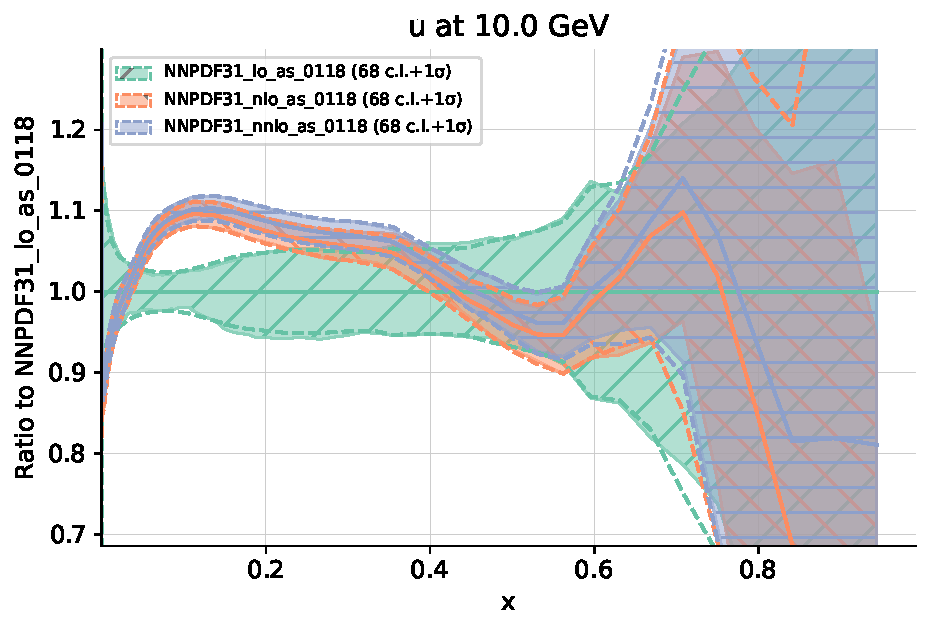
\includegraphics[width=0.49\linewidth]{mhous/plots/pdfscalespecs1_basespecs0_pdfnormalize1_plot_pdfs_u.pdf}
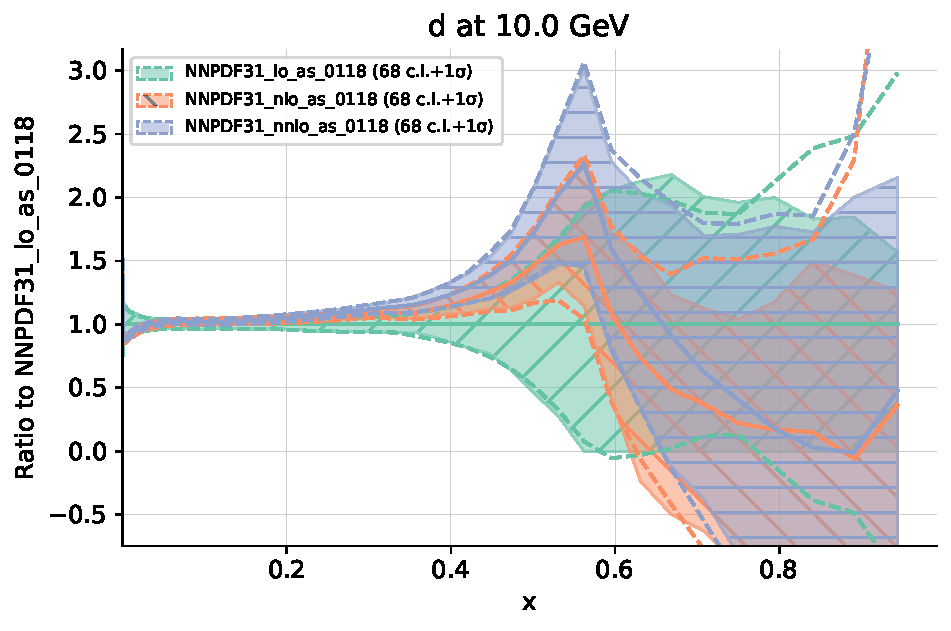
\includegraphics[width=0.49\linewidth]{mhous/plots/pdfscalespecs1_basespecs0_pdfnormalize1_plot_pdfs_d.pdf}\\
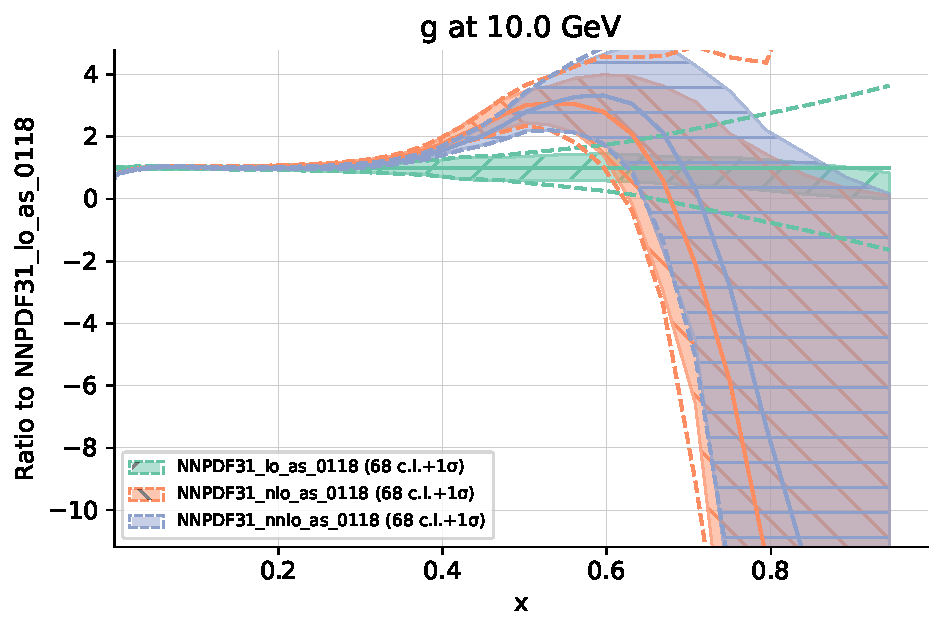
\includegraphics[width=0.49\linewidth]{mhous/plots/pdfscalespecs1_basespecs0_pdfnormalize1_plot_pdfs_g.pdf}
\caption{Comparison of NNPDF3.1 PDFs at different perturbative orders: LO (green); NLO (orange); NNLO (blue). PDFs are normalised to the LO result, and displayed at scale $Q$ = 10 GeV.}
\label{fig:pdf_order_comp}
\end{figure}

In addition to a missing source of per-point uncertainty on each data point, MHOUs can affect a PDF fit more insidiously by impacting on the desired weight of data sets relative to one another; regions of data with high MHOU are naturally to be trusted less when used to determine the PDFs, and so should carry less weight in the fitting process. If MHOUs are included, these data will be deweighted automatically because they will carry higher uncertainty, however in the absence of MHOUs they may impact on a fit to an undesirable degree.

Having established the importance of including MHOUs, in the next section we will go on to develop a formalism for estimating them, and constructing a MHOU covariance matrix.

\section{Scale variation}
\label{sec:svn}

The most popular method for estimating MHOUs is by ``scale variation". This is based on making theoretical predictions at a range of values of the artificial renormalisation ($\mu_R$) and factorisation ($\mu_F$) scales introduced in Chapter~\ref{chapter:background}. The renormalisation group equation (RGE;~\ref{eqn:rge}) and factorisation theorem only hold to all orders in perturbation theory, and in this case varying the scale values will have no effect on any results. However, when the perturbative expansion is truncated, there will be a residual $\mu_R$ and $\mu_F$ dependence which characterises the degree of MHOU. Varying these scales and observing the impact on the predictions can therefore provide an estimate of the MHOUs. 

Although other approaches to estimating MHOUs, based on the current known orders, have been suggested~\cite{Cacciari:2011ze, David:2013gaa, Bagnaschi:2014wea}, we adopted the method of scale variations not only because it is the most widely used, but also because it is the most easily implemented for our purposes. Firstly, the renormalisation group invariance is incorporated automatically, which ensures the MHOUs decrease as the perturbative order increases. Secondly, the scale dependece of $\alpha_s(\mu_R^2)$ and the PDFs is universal to all processes, which is important for PDF fits dealing with a range of interactions. Finally, correlations between data points are implicitly maintained because predictions for different scale values will be smooth functions of kinematics; this ensures that neighbouring regions of phase space will be strongly correlated.

There are, however, some disadvantages. Firstly, the definition of the two scales themselves have been historically approached in various ways, often differently for DIS and hadronic collisions, but also changing over time. Since PDFs use both DIS and hadronic data we need to settle on a consistent approach. Secondly, there is no cut and dry method for determining the range of varied scale choices, and in fact the choice of central scales are themselves to some degree arbitrary; for example, top production processes commonly have both central scales set to the top mass, $m_t$, and DIS processes have both set to Bj\"orken $Q$. Though there is physical motivation for these choices, we could equally well pick 2$m_t$ rather than $m_t$ in the former case, for example. A standard approach is to take the 7-point envelope of the predictions obtained by varying $(\mu_F, \mu_R)$ independently in $\{1/2, 1, 2\}$, excluding $(1/2, 1/2)$ and $(2,2)$. However, for our purposes we do not want a per-point envelope but rather a covariance matrix which retains correlations between data points. We will address both of these drawbacks below. 

Finally, scale variation techniques will not pick up any ``new physics" at higher orders, be it additional colour configurations, singularities or mechanisms of interaction. This is harder to deal with, and requires resummation techniques among other methods. In this work we assume these effects to be less important, and do not address them for the time being.

In the remainder of this section we will review the technique of scale variation, and with it the definitions of $\mu_F$ and $\mu_R$. We will converge on a genral formalism that can be applied to both electroproduction and hadroproduction. We will show that there are two independent directions of scale variation and discuss how to combine them, both in single process and multi-process interactions. We will then go on to show how to use this to build a covariance matrix in Sec.~\ref{sec:prescrip}.

\subsection{Renormalisation group invariance}

It is customary when making a theory prediction to pick a renormalisation scale, $\mu_R$, that is indicative of the physical scale of the interaction, $Q$. We will denote this ``central" theory prediction by $T(Q^2)$. In general, a theory prediction at scale $\mu_R$ can be written
$\overline{T}(\alpha_s(\mu_R^2), \mu_R^2/Q^2)$, where we explicitly note that $\alpha_s$ itself depends on the renormalisation scale. From this we can see that
\beq
T(Q^2) \equiv \overline{T}\big(\alpha_s(Q^2), 1 \big).
\eeq
The strong coupling constant satisfies the RGE
\beq \label{eqn:beta}
\mu_R^2 \frac{d^2}{d\mu_R^2}\alpha_s(\mu_R^2) = \beta \big( \alpha_s (\mu_R^2) \big),
\eeq
and we can expand the beta function perturbatively as
\beq 
\beta(\alpha_s) = \beta_0 \alpha_s^2 + \beta_1 \alpha_s^3 
+ \beta_2 \alpha_s^4 + \ldots \, .
\eeq

As discussed in Chapter~\ref{chapter:background}, renormalisation group invariance tells us that a prediction of a physical quantity (such as $\overline{T}$) to all orders must be independent of $\mu_R$, because this scale is unphysical. This means we can write
\beq \label{eqn:rgetbar}
  \mu_R^2 \frac{d}{d \mu_R^2} \overline{T} \lp
  \alpha_s(\mu_R^2), \mu_R^2/Q^2\rp  = 0 .
\eeq

Before proceeding further, we introduce some variables to make the analysis clearer:
\beq \label{eqn:notn}
\mu_R^2 = k Q^2,\qquad t = \ln (Q^2 / \Lambda^2), \qquad \kappa = \ln k = \ln \mu_R^2/Q^2,
\eeq
where $\Lambda$ is the QCD scale. This means $\alpha_s(\mu_R^2)$ is a function of $\ln \mu_R^2/\Lambda^2 = t + \kappa$.

Revisiting Eqn.~\ref{eqn:rgetbar}, we can write this as
\bea \label{eqn:newrge}
	0 & =& \frac{d}{d \kappa} \overline{T}(\alpha_s(t + \kappa), \kappa) \nonumber\\
	& =& \frac{d} {d \kappa} \alpha_s(t + \kappa) \frac{\partial}{\partial \alpha_s} \overline{T}(\alpha_s(t + \kappa), \kappa) \bigg|_\kappa + \frac{\partial}{\partial \kappa} \overline{T}(\alpha_s(t + \kappa), \kappa) \bigg|_{\alpha_s}\nonumber, \\
\eea
assuming that $\overline{T}$ is analytic in $\alpha_s$ and $\kappa$. To simplify this we can use
\beq 
	\frac{d}{d \kappa} \alpha_s(t + \kappa) = \frac{d}{dt} \alpha_s(t + \kappa) = \frac{d}{d \ln \mu_R^2} \alpha_s(t + \kappa) = \beta(\alpha_s(t + \kappa) ) \, ,
\eeq
where we have used the definition of the beta function (Eqn.~\ref{eqn:beta}), and this means that
\beq
	0 = \frac{\partial}{\partial t} \overline{T}(\alpha_s(t + \kappa), \kappa) \bigg|_\kappa + \frac{\partial}{\partial \kappa} \overline{T}(\alpha_s(t + \kappa), \kappa) \bigg|_{\alpha_s} \, .
\eeq
We can now Taylor expand $\overline{T}(\alpha_s, \kappa)$ about the central scale $\mu_R^2 = Q^2 \implies k=1 \implies \kappa = 0$ for fixed $\alpha_s$: 
\bea
  \overline{T}(\alpha_s(t + \kappa), \kappa) &=& \overline{T}(\alpha_s(t + \kappa), 0)\nonumber\\&&\qquad\qquad +\kappa \frac{\partial}{\partial \kappa} \overline{T}(\alpha_s(t + \kappa), 0) \bigg|_{\alpha_s} + \half \kappa^2 \frac{\partial^2}{\partial \kappa^2} \overline{T}(\alpha_s(t + \kappa, 0)\bigg|_{\alpha_s} + \ldots \qquad \nonumber \\.
\eea
Then, using Eqn.~\ref{eqn:newrge}, we can replace $\frac{\partial}{\partial \kappa}$ with
$-\frac{\partial}{\partial t}$, and write
\bea \label{eqn:trelation}
\overline{T}(\alpha_s(t + \kappa), \kappa) &=& \overline{T}(\alpha_s(t + \kappa), 0) - \kappa \frac{\partial}{\partial t} \overline{T}(\alpha_s(t + \kappa), 0) \bigg|_\kappa \nonumber\\ &+& \half \kappa^2  \frac{\partial^2}{\partial t^2} \overline{T}(\alpha_s(t + \kappa), 0)\bigg|_\kappa + \ldots \nonumber\\
&=& T(t + \kappa) - \kappa \frac{d}{dt} T(t + \kappa) + \half \kappa^2  \frac{d^2}{dt^2} T(t + \kappa)+\ldots\>.
\eea
This tells us how to find a scale varied theoretical prediction, $\overline{T}$, in terms of the $t$ dependence of the central prediction, $T$. Furthermore, we can express this $t$ dependence as an $\alpha_s$ dependence using
\beq
\frac{d}{dt} T(t) = \frac{d \alpha_s(t)}{dt} \frac{\partial}{\partial \alpha_s} \overline{T}(\alpha_s(t), 0) = \beta(\alpha_s(t)) \frac{\partial}{\partial \alpha_s} \overline{T}(\alpha_s(t), 0).
\eeq
Noting that $\beta(\alpha_s) = \mathcal{O}(\as^2)$, we see that 
$\frac{1}{T} \frac{dT}{dt}
= \mathcal{O}(\alpha_s)$ and $\frac{1}{T} \frac{d^2T}{dt^2} =
\mathcal{O}(\alpha_s^2)$ etc. The pattern follows that every time a derivative is taken with respect to $t$ you pick up a power of $\alpha_s$ as a consequence of the chain rule in differentiating. Looking back at Eqn. \ref{eqn:trelation} it is clear that each power of $\kappa$ is associated with a power of $\alpha_s$. Expressing the theory prediction perturbatively as
\be
T = \alpha_sT_{\text{LO}} + \alpha_s^2 T_{\text{NLO}} + \alpha_s^3 T_{\text{NNLO}} + \ldots\> ,
\ee
we can match powers of $\alpha_s$ in Eqn. \ref{eqn:trelation} to obtain the expressions
\begin{align} \label{eqn:theoryshifts}
\begin{split}
	\overline{T}_{\text{LO}}(\alpha_s(t + \kappa), \kappa) & = T_{\text{LO}}(t + \kappa), \\
	\overline{T}_{\text{NLO}}(\alpha_s(t + \kappa), \kappa) & = T_{\text{NLO}}(t + \kappa) - \kappa\smallfrac{d}{dt}{T}_{\text{LO}}(t + \kappa), \\
	\overline{T}_{\text{NNLO}}(\alpha_s(t + \kappa), \kappa) & = T_{\text{NNLO}}(t + \kappa) - \kappa\smallfrac{d}{dt}{T}_{\text{NLO}}(t + \kappa) \\
	&+ \half\kappa^2  \smallfrac{d^2}{dt^2}{T}_{\text{LO}}(t + \kappa).
\end{split}
\end{align}

The difference between the scale varied prediction and the central scale prediction,
\be
\Delta(t,\kappa) = \overline{T}(\alpha_s(t + \kappa), \kappa) - T(t) \, .
\ee
can be used to estimate the MHOU. From Eqn.~\ref{eqn:theoryshifts} we find the explicit expressions for the theory uncertainties
\be 
\begin{split}
\Delta_{\text{LO}}(t,\kappa) & = T_{\text{LO}}(t + \kappa)-T_{\text{LO}}(t), \\
{\Delta}_{\text{NLO}}(t,\kappa) & = (T_{\text{NLO}}(t + \kappa) - \kappa\smallfrac{d}{dt}{T}_{\text{LO}}(t + \kappa))-T_{\text{NLO}}(t), \\
{\Delta}_{\text{NNLO}}(t, \kappa) & = (T_{\text{NNLO}}(t + \kappa) - \kappa\smallfrac{d}{dt}{T}_{\text{NLO}}(t + \kappa) \\
&+ \half\kappa^2  \smallfrac{d^2}{dt^2}{T}_{\text{LO}}(t + \kappa))-T_{\text{NNLO}}(t) \, .
\end{split}
\ee
At LO we can see that the uncertainty results entirely from the choice of $\kappa$, in other words of $\mu_R$ in the $\alpha_s$ evaluation. At NLO we can see that the leading part of $T_{\text{NLO}}(t + \kappa)$ is subtracted off by the $\mathcal{O}(\kappa)$ term, meaning that the uncertainty is reduced with respect to LO. At NNLO, in addition, the $\mathcal{O}(\kappa^2)$ term subtracts off the subleading dependence of $T_{\text{NNLO}}(t + \kappa) - \kappa\smallfrac{d}{dt}{T}_{\text{NLO}}(t + \kappa)$, and so the uncertainty is yet smaller. This pattern of decreased scale variation uncertainties with increased perturbative order reflects our general understanding of the behaviour of MHOUs.

It is also apparent that the size of MHOU depends on the value of $\kappa$, in other words on the size of scale variation. This introduces a degree of arbitrariness into MHOU estimation, with the historical empirical range of choice being $\kappa \in [-\ln 4, \ln 4]$. In practice, we must investigate the dependence of $\Delta$ on $\kappa$, using validation at lower orders against known higher orders to converge on a suitable prescription.  This will be addressed in Sec.~\ref{sec:prescrip}. 

We will now go on to show how RG invariance can be applied to processes involving hadrons, where the partonic cross section is also convolved with a PDF. We will show that in this scenario there are two independent scales, and thus two independent sources of MHOU: one from the $\alpha_s$ dependence in the hard cross section; the other from the anomalous dimensions in the PDF evolution.

\subsection{Scale variation in partonic cross sections}
\label{subsec:svpartonic}
We will start with DIS, where there is only one hadron then move to the case of hadron-hadron collisions, such as those carried out at the LHC. In each case we will consider RG invariance to find an expression for $\mu_R$ variation in the partonic observable, for the case where the PDF is evaluated at the physical scale. Scale variation in PDF evolution, i.e. the $\mu_F$ variation, will be addressed in the next section.
\subsubsection{Deep Inelastic Scattering}
For DIS processes, theory predictions are of the structure functions discussed in Chapter~\ref{chapter:background}. These can be expressed as a convolution of a parton level coefficient, $C$, with a PDF, $f$:
\be 
\label{eqn:strfn}
F(Q^2) = C(x, \alpha_s(Q^2)) \otimes f(x, Q^2),
\ee
where $\otimes$ is a convolution in the momentum fraction, $x$, and there is an implicit sum over parton flavours. There will be a MHOU in $F$ due to truncating the coefficient function, $C$, to fixed perturbative order.  We can estimate this by keeping the PDF scale (or factorisation scale) fixed and varying the renormalisation scale in $C$. This will result in a scale-varied structure function,
\be
    \overline{F}(Q^2, \mu_R^2) = \overline{C}(\alpha_s(\mu_R^2), \mu_R^2/Q^2)\otimes f(Q^2)\, ,
\ee
where we have made the $x$-dependence implicit and the scale dependence explicit in the coefficient function. We can use the quantities defined in Eqn.~\ref{eqn:notn} to write this as
\be 
    \overline{F}(t, \kappa) = \overline{C}(\alpha_s(t + \kappa), \kappa)\otimes f(t).
\ee
We know that the structure function, an observable, is RG invariant, and, because we are keeping the factorisation scheme fixed, the PDF is independent of $\mu_R$. This means that the coefficient functions must also obey RG invariance, and so in a parallel with Eqn.~\ref{eqn:trelation} we can write
\be	
\overline{C}(\alpha_s(t + \kappa), \kappa) = C(t + \kappa) - \kappa \smallfrac{d}{dt} C(t + \kappa) + \half \kappa^2  \smallfrac{d^2}{dt^2} C(t + \kappa)+\ldots,
\ee
where, like before, we denote the central scale quantities without a bar. In order to evaluate the derivatives, note that the coefficient function can be expressed as a perturbative expansion in $\alpha_s$,
\be 
C(t) = c_0 + \alpha_s(t) c_1 + \alpha_s^2(t) c_2 + \alpha_s^3(t) c_3 +\ldots, 
\ee
and that $\smallfrac{d}{dt}\alpha_s(t,\kappa) = \beta(\alpha_s(t, \kappa)$, where the beta function also admits the expansion in Eqn.~\ref{eqn:beta}. Explicitly, this leads us to
\be 
\begin{split}
\smallfrac{d}{dt}{C}(t) & = \alpha_s^2(t) \beta_0 c_1+ \alpha_s^3(t) (\beta_1c_1+2\beta_0c_2) + \ldots,\\
\smallfrac{d^2}{dt^2}{C}(t) & = 2\alpha_s^3(t) \beta_0^2 c_1+ \ldots,
\end{split}
\ee 
resulting in the perturbative expression for $\mu_R$ variation of $C$:
\be 
\begin{split}
\overline{C}(\alpha_s(t + \kappa), \kappa) = c_0 &+ \alpha_s(t + \kappa) c_1 + \alpha_s^2(t + \kappa) (c_2 - \kappa \beta_0 c_1)\\ 
&+\alpha_s^3(t + \kappa)\big(c_3-\kappa (\beta_1c_1+2\beta_0c_2)+ \kappa^2 \beta_0^2 c_1\big) + \ldots \, .
\end{split}
\ee 
Using Eqn.~\ref{eqn:strfn} we finally get an expression for the $\mu_R$ variation of $F$:
\be 
\begin{split}
\overline{F}(t, \kappa) = c_0\otimes f(t) &+ \alpha_s(t + \kappa) c_1\otimes f(t) + \alpha_s^2(t + \kappa)  \lp c_2 - \kappa \beta_0 c_1 \rp \otimes f(t)\\ 
&+\alpha_s^3(t + \kappa) \lp c_3-\kappa (\beta_1c_1+2\beta_0c_2)+ \kappa^2 \beta_0^2 c_1 \rp \otimes f(t) + \ldots\>. 
\end{split}
\ee.
In practice, when predicting scale varied observables, using these equations is relatively straightforward. Because the coefficients, $c_i$ and $\beta_i$, are already known to some order, the workflow consists of some basic algebra to create the new, scale varied, coefficients at each order from the central-scale coefficients at the surrounding orders.

\subsubsection{Hadron-hadron collisions}
Hadron-hadron collisions can be considered in a similar way to DIS, the difference being that the observable cross section, $\Sigma$, depends on two PDFs, one for each of the hadrons:
\be 
    \Sigma(t) = H(t)\otimes( {f}(t)\otimes  {f}(t)) \, ,
\ee
where $H$ is the parton level cross section and this time we have used $t = \ln (Q^2 / \Lambda^2)$ from the outset. Once again, there is an implicit sum over parton flavours. As before, we can vary $\kappa = \ln (\mu^2/Q^2)$ in $H$ whilst keeping $f$ fixed, so that
\be \label{eqn:svarhadronic}
  \overline{\Sigma}(t,\kappa) = \overline{H} (\as(t+\kappa), \kappa)\otimes(f(t)\otimes f(t)),
\ee 
where
\be 
\overline{H}(\alpha_s(t), \kappa) = H(t) - \kappa \smallfrac{d}{dt} H(t) + \half \kappa^2  \smallfrac{d^2}{dt^2} H(t)+\ldots\>. 
\ee
Because hadron-hadron collisions involve a range of processes, we consider a generic process starting at $O(\alpha_s^n)$ for $n \in \mathbb{Z}$, so that
\be 
H(t) = \alpha_s^n(t)h_0 + \alpha_s^{n+1}(t)h_1 + \alpha_s^{n+2}(t)h_2+ \ldots\>.
\ee
Once again using $\smallfrac{d}{dt}\alpha_s(t,\kappa) = \beta(\alpha_s(t, \kappa)$ and Eqn.~\ref{eqn:beta} we arrive at
\begin{equation}
\begin{split}
\smallfrac{d}{dt}{H}(t) & = n\alpha_s^{n-1}(t)\beta(\alpha_s) h_0 + (n+1)\alpha_s^n(t)\beta(\alpha_s) h_1 + \ldots \\
&= \alpha_s^{n+1} n \beta_0 h_0 + \alpha_s^{n+2} (n \beta_1 h_0 + (n+1) \beta_0 h_1) + \ldots\\
\smallfrac{d^2}{dt^2}{H}(t) & = \alpha_s^{n+2} n(n+1) \beta_0^2 h_0 + \ldots.
\end{split}
\end{equation}
Overall, to evaluate $\overline{\Sigma}$ we can therefore use Eqn.~\ref{eqn:svarhadronic} along with 
\bea  \label{eqn:svarH}
    \overline{H}(\alpha_s, \kappa) &=& \alpha_s^n h_0 + \alpha_s^{n+1} (h_1 - \kappa n \beta_0 h_0) \nonumber\\ &+&\alpha_s^{n+2} (h_2 - \kappa(n \beta_1 h_0 + (n+1) \beta_0 h_1) \nonumber\\ &&\qquad+ \half \kappa^2 n(n+1) \beta_0^2 h_1) + \ldots .
\eea
Again, to evaluate the scale varied cross section, all that is needed is to modify the coefficients at each order using those at the central scale for the surrounding orders.
\subsection{Scale variation in evolution of PDFs}
We now turn to the effects of scale variation in the PDFs themselves. This is a crucial contribution to MHOUs because the PDFs are common to predictions for all processes, and therefore responsible for widespread correlations in uncertainty. MHOUs in the PDFs arise from the truncation of the perturbative expansion of the splitting functions (or, in Mellin space, the anomalous dimensions) in the DGLAP evolution equations (Eqn.~\ref{eqn:DGLAP}) discussed in Chapter~\ref{chapter:background}. The scale evolution of the PDFs can be encapsulated in Mellin space in the equation
\be \label{eqn:mellindglap}
	\mu_F^2 \frac{d}{d \mu_F^2} f(\mu_F^2) = \gamma(\alpha_s(\mu_F^2)) f(\mu_F^2)\, ,
\ee
where the parton flavour indices are left implicit and the anomalous dimension, $\gamma$, can be expressed as an expansion in $\alpha_s$ as
\be  \label{eqn:anomdimexp}
\gamma(t) =  \alpha_s(t) \gamma_0 + \alpha_s^2(t) \gamma_1^2  + \alpha_s^3(t) \gamma_2^3 + \cdots .
\ee
Note that we refer to a separate factorisation scale, $\mu_F$, distinct from the renormalisation scale, $\mu_R$, in the previous section. This is because each scale is associated with a separate RGE and they are therefore independent; to explore the full space of scale variations they need to be considered separately. 

To solve for the PDF, we can integrate Eqn.~\ref{eqn:mellindglap} to give
\be \label{eqn:pdfint}
	f(\mu_F^2) = \text{exp}\bigg(\int_{\mu_0}^{\mu_F^2} \frac{d \mu^{2}}{\mu^{2}} \gamma(\alpha_s(\mu^{2}))\bigg) f_0 \, ,
\ee
where $f_0$ is the PDF at the initial scale, $\mu_0$. Note that the LHS is independent of the choice of $\mu_0$. To consider the effect of scale variations on the PDF, we can proceed similarly to Sec.~\ref{subsec:svpartonic}, defining 
\beq \label{eqn:notn2}
\mu_F^2 = k Q^2,\qquad t = \ln (Q^2 / \Lambda^2), \qquad \kappa = \ln k = \ln \mu_F^2/Q^2,
\eeq
and finding the scale varied anomalous dimension
\be \label{eqn:svanomdim}
	\overline{\gamma}(\alpha_s(t), \kappa) = \gamma(t) - \kappa
        \smallfrac{d}{dt}{\gamma}(t) + \half \kappa^2
        \smallfrac{d^2}{dt^2}{\gamma}(t) + \cdots .
\ee
Once again we can use the beta function expansion (Eqn.~\ref{eqn:beta}) alongside Eqn.~\ref{eqn:anomdimexp} to give
\bea \label{eqn:anomdimresult}
    \overline{\gamma}(\alpha_s(t + \kappa), \kappa) &=& \alpha_s(t+\kappa) \gamma_0 + \alpha_s^2(t+\kappa) (\gamma_1 - \kappa \beta_0 \gamma_0) \nonumber\\ &+& \alpha_s^3(t+\kappa) (\gamma_2 - \kappa (\beta_1 \gamma_0 + 2 \beta_0 \gamma_1) + \kappa^2 \beta_0^2 \gamma_0) \nonumber\\ &+& \cdots \, ,
\eea
which has the same form as Eqn.~\ref{eqn:svarH} upon setting $n=1$. We can use this equation to estimate MHOUs in PDFs, which can be done by refitting the PDF at each scale choice using different anomalous dimensions. This method has been applied in previous analyses~\cite{Martin:1990fq, Virchaux:1991jc, Ridolfi:1999vr}, but the process of refitting the PDFs is computationally intensive and so we would like to avoid having to do this if possible. Instead, we can look directly at the PDF level and consider evaluating the PDFs themselves at different scales, as was done in Ref.~\cite{Altarelli:2008aj}.  

We can define the scale varied PDF as that obtained by varying the scale in the anomalous dimension,
\be
\overline{f}(\as(t + \kappa), \kappa) = \text{exp}\bigg(\int_{t_0}^t dt' \overline{\gamma}(\alpha_s(t' + \kappa), \kappa)\bigg) f_0 \, 
\ee
Shifting integration variable $t' \to t'- \kappa$ whilst redefining the initial scale, we can then apply Eqn.~\ref{eqn:svanomdim} and expand the exponential, {\it i.e.}
\bea
\overline{f}(\as(t + \kappa), \kappa) &=& \text{exp}\bigg(\int_{t_0}^{t+\kappa} dt' \overline{\gamma}(\alpha_s(t'), \kappa)\bigg) f_0 \nonumber\\
&=& \exp\lp \lc \int_{t_0}^{t + \kappa} dt' \gamma(t')\rc  - \kappa  \gamma(t + \kappa) + \half \kappa^2 \frac{d}{dt} {\gamma}(t + \kappa) + \ldots \rp \nonumber\\
&& \times \exp\lp \kappa  \gamma(t_0) - \half \kappa^2 \frac{d}{dt} {\gamma}(t_0) + \ldots \rp f_0 \\
&=& \lc 1 - \kappa \gamma(t + \kappa) + \half \kappa^2
    (\gamma^2(t + \kappa)+\frac{d}{dt}{\gamma}(t + \kappa)) + \ldots
    \rc \nonumber\\
&& \times \exp\lp \int_{t_0}^{t + \kappa} dt' \gamma(t')\rp \exp\lp \kappa  \gamma(t_0) - \half \kappa^2 \frac{d}{dt} {\gamma}(t_0) + \ldots \rp f_0 \nonumber \, .
\eea
We can absorb the factor resulting from variation of $t_0$ into the initial PDFs, $f_0$, so that $\exp\lp \kappa  \gamma(t_0) - \half \kappa^2 \frac{d}{dt} {\gamma}(t_0) + \ldots \rp f_0 \to f_0$. Then, noting also that $\exp\lp \int_{t_0}^{t + \kappa} dt' \gamma(t')\rp f_0 = f(t + \kappa)$, we end up with the result
\be \label{eqn:pdfvarresult}
\overline{f}(\as(t + \kappa), \kappa) = \lc 1 - \kappa \gamma(t + \kappa) + \half \kappa^2
    (\gamma^2(t + \kappa)+\frac{d}{dt}{\gamma}(t + \kappa)) + \ldots
    \rc f(t+ \kappa) \, .
\ee
This result, which comes from varying the scale at which the PDF is evaluated, is equivalent to the result which comes from varying the scale in the anomalous dimension, Eqn.~\ref{eqn:anomdimresult}. This is because there is only one RGE and therefore only one scale which the PDF depends on. Furthermore, note that Eqn.~\ref{eqn:pdfvarresult} shows us that the scale dependence can be factorised out of the PDF. This means we are free to instead factor it into the parton level coefficient function, which will always appear convolved with the PDF. This is useful when making a scale varied prediction when only a central PDF is available, and has been used in the past to make predictions for new LHC processes (e.g. Higgs production~\cite{deFlorian:2016spz}). However, in the case where we also want to consider $\mu_R$ variation in the coefficient function, the two scale variations will be mixed up, and this can lead to a complicated interplay, especially in the presence of heavy quark effects. In this work we adopt the method of scale variation for PDFs by using Eqn.~\ref{eqn:pdfvarresult}. 

\subsection{Varying two scales together}
We now consider the simultaneous variation of $\mu_R$ in the parton level observable and $\mu_F$ in the PDFs, in order to explore the full range of scale variation space. We will derive formulae for scale variation up to NNLO which are needed to construct a MHOU covariance matrix. 

For a DIS process we can write the double-scale-varied structure function as
\be \label{eqn:doublesv}
\overline{F}(Q^2, \mu_F^2, \mu_R^2) = \overline{C}(\alpha_s(\mu_R^2), \mu_R^2/Q^2) \otimes \overline{f}(\alpha_s(\mu_F^2), \mu_F^2/Q^2).
\ee
Similarly to before, we can define the variables
\beq \label{eqn:notn3}
\mu_{(F/R)}^2 = k_{(F/R)} Q^2,\qquad \kappa_{(F/R)} = \ln k_{(F/R)}, \qquad t_{(F/R)} = t + \kappa_{(F/R)}
\eeq
and use them to write the structure function as
\be
    \overline{F}(t, \kappa_F, \kappa_R) = \overline{C}(t_R, \kappa_R)
    \overline{f}(t_F, \kappa_F).
\ee
We then need to apply the equations for the scale varied PDFs and coefficient functions from the previous section, 
\be 
\begin{split}
    &\overline{f} (t_F, \kappa_F) = f(t_F) - \kappa_F
  \smallfrac{d}{dt}{f}(t_F) + \half \kappa_F^2
  \smallfrac{d^2}{dt^2}{f}(t_F) + ... \, , \\ 
    &\overline{C} (t_R, \kappa_R) = C(t_R) - \kappa_R
  \smallfrac{d}{dt}{C}(t_R) + \half \kappa_R^2
  \smallfrac{d^2}{dt^2}{C}(t_R) + ...   \, ,
\end{split}    
\ee
and use the fact that $\smallfrac{\partial}{\partial t} \sim \mathcal{O}(\alpha_s)$ to see that
\bea
    \overline{F}(t, \kappa_F, \kappa_R) 
    &=& C(t_R)f(t_F) - \lp \kappa_F C(t_R) \smallfrac{d}{dt}{f} (t_F)
    + \kappa_R \smallfrac{d}{dt}{C}(t_R) f(t_F) \rp  \nonumber\\
    &&\qquad + \half\Big(  \kappa_F^2
    C(t_R) \smallfrac{d^2}{dt^2} f(t_F)  
    + 2\kappa_R \kappa_F
    \smallfrac{d}{dt}{C}(t_R)\smallfrac{d}{dt}{f}(t_F) \nonumber\\
    &&\qquad \qquad +
    \kappa_R^2 \smallfrac{d^2}{dt^2}{C}(t_R)f(t_F)\Big) +
    \mathcal{O}(\alpha_s^3) \, . 
\eea
Taking a closer look, and comparing to Eqn.~\ref{eqn:doublesv}, we can write this in terms of partial derivatives of $F$:
\bea
    \overline{F}(t, \kappa_F, \kappa_R)  &=& F(t_F,t_R) - \bigg( \kappa_F\ \frac{\partial F}{\partial t_F}\bigg|_{t_R} + \kappa_R\ \frac{\partial F}{\partial t_R}\bigg|_{t_F} \bigg) \nonumber\\
    &&\qquad+ \half \bigg( \kappa_F^2 \frac{\partial^2 F}{\partial t_F^2}\bigg|_{t_R} +  2 \kappa_F \kappa_R \frac{\partial^2 F}{\partial t_F \partial t_R} \nonumber \\ &&\qquad +  \kappa_R^2 \frac{\partial^2 F}{\partial t_R^2}\bigg|_{t_F} \bigg)  + \cdots \, .    
\eea
Considering this expression, we can think of $\kappa_F\smallfrac{\partial}{\partial t_F}$ and $\kappa_R\smallfrac{\partial}{\partial t_R}$ as being the generators of the two types of scale variations.

For hadronic-hadron processes, the double-scale-varied cross section is instead
\be 
\overline{\Sigma}(t_F, t_R, \kappa_F, \kappa_R) = \overline{H}(\as(t_R), \kappa_R)\otimes  \lp \overline{f}(t_F, \kappa_F)\otimes\overline{f}(t_F, \kappa_F) \rp \, .
\ee
and we can apply exactly the same approach as above, leading to 
\bea
    \overline{\Sigma}(t, \kappa_F, \kappa_R)  &=& \Sigma(t_F,t_R) - \bigg( 2\kappa_F\ \frac{\partial \Sigma}{\partial t_F}\bigg|_{t_R} + \kappa_R\ \frac{\partial \Sigma}{\partial t_R}\bigg|_{t_F} \bigg) \nonumber\\
    &&\qquad+ \half \bigg( 2\kappa_F^2 \frac{\partial^2 \Sigma}{\partial t_F^2}\bigg|_{t_R} +  4 \kappa_F \kappa_R \frac{\partial^2 \Sigma}{\partial t_F \partial t_R} \nonumber \\ &&\qquad +  \kappa_R^2 \frac{\partial^2 \Sigma}{\partial t_R^2}\bigg|_{t_F} \bigg)  + \cdots \, ,    
\eea
where this time we pick up a factor of 2 with each $\kappa_F\smallfrac{\partial}{\partial t_F}$, due to the two PDFs.
\subsection{Scale variation for two processes}
We are now approaching a formalism which can be applied to carry out scale variations for the data included in PDF fits. But first we need to work out how to carry out simultaneous scale variations involving data from more than one process, for example DIS and Drell-Yan. Because the theory covariance matrix contains correlations between each two data points, carrying out simultaneous scale variations for two processes is sufficient because we only need to consider two data points at a time. 

For the case of two separate processes, the parton level cross sections will be totally independent, so there will be two separate RGEs and therefore two separate renormalisation scales, and hence renormalisation scale variation should be uncorrelated. However, all the processes share a common factorisation scale, and so the factorisation scale variation must be correlated.

\section{Building the theory covariance matrix}
\label{sec:prescrip}
\subsection{Symmetric prescriptions}
\subsection{Asymmetric prescriptions}
\subsection{Categorising processes}
\subsection{NLO theory covariance matrices}

\section{Validating the theory covariance matrix}
\label{sec:valid}

\section{PDFs with missing higher order uncertainties}
\label{sec:pdfs}

\section{Impact on phenomenology}
\label{sec:mhoupheno}
